% Appendix D — hydride candidates (DFT-sourced, absorbed=false). \input'd by main.tex.
\section{Hydride Candidates --- DFT-Sourced, \texttt{absorbed=false}}
\label{app:hydride}

This appendix is the full data record for the candidate-material axis,
pipeline stages \textcircled{\scriptsize 1}--\textcircled{\scriptsize 2}:
the binary and ternary hydride candidates whose
$\lambda,\omega_{\log},\mu^{*}$ are \emph{sourced} from external
electron--phonon DFT, never re-derived here. It states the
stability$\leftrightarrow$strong-coupling wall and records the candidates
as \texttt{absorbed=false} with the high-pressure / replication boundary
explicit. \textbf{No room-temperature superconductor is claimed here.}
Candidate slate (sourced): SrAuH$_3$, LaBeH$_8$, YSbH$_6$, the
binary-hydride sweep (h3cl / h3o / h3si / h3po / H$_3$As), plus the
H$_3$S / CaH$_6$ measured anchors.

% -------------------------------------------------------------------------
\subsection{The stability $\leftrightarrow$ strong-coupling wall}
\label{app:hyd-wall}

The recurring physical obstruction across the whole hydride family is a
trade-off: the large electron--phonon coupling $\lambda$ that lifts $T_c$
(Appendix~\ref{app:allendynes}) comes from soft, anharmonic phonon modes
--- and a mode soft enough to give high $\lambda$ is, at accessible
pressure, often soft enough to go \emph{imaginary} (dynamically unstable).
The binary-hydride sweep (RTSC.md \S9.16, ``N5 sweep CLOSED as wall'') made
this concrete:
\begin{itemize}\itemsep0.2em
\item \textbf{Stable but low-$T_c$}: SrAuH$_3$ ($\lambda\!=\!0.62
  \Rightarrow T_c\!=\!14.6$\,K, PR~\#91), h3si ($T_c\!=\!78$\,K),
  h3br ($\sim\!110$\,K) --- dynamically stable, but $T_c\!<\!200$\,K.
\item \textbf{High-$\lambda$ but unstable}: H$_3$As ($\lambda\!\to\!1.0$
  but dynamically unstable, PR~\#97), h3po (unstable) --- the coupling is
  there, the structure is not.
\item \textbf{High both, only at megabar}: H$_3$S ($\sim$203\,K,
  \citep{drozdov2015}), CaH$_6$ ($\lambda\!=\!3.40$--$4.38$) --- clear
  $T_c$, but only at $\sim$150--200\,GPa, where the material is not a
  device.
\end{itemize}
The bisection is the load-bearing finding: \textbf{no surveyed candidate
sits in the upper-right ``stable AND $T_c\!>\!200$\,K AND ambient''
quadrant}. The binary axis is declared exhausted for RTSC; the ternary
cation-stuffed family (Mg$_2$IrH$_6$ $\sim$160\,K predicted ambient,
Li$_2$CuH$_6$ $\sim$86\,K, LaBeH$_8$ 110\,K measured-anchor) is the open
N6 funnel --- whether cation decoupling escapes the dynamical-stability
($m\!>\!0$) gate at ambient pressure is the live first-principles question.

% -------------------------------------------------------------------------
\subsection{Candidate slate (sourced)}
\label{app:hyd-table}

\begin{table}[h]
\centering
\small
\setlength{\tabcolsep}{4.5pt}
\begin{tabular}{@{}lrrrcccc@{}}
\toprule
\textbf{Compound} & $\boldsymbol{\lambda}$ & $\boldsymbol{\omega_{\log}}$\,(K)
& $\boldsymbol{T_c}$\,(K) & \textbf{Pressure} & \textbf{Dyn.\,stable?}
& \textbf{absorbed} & \textbf{Source} \\
\midrule
SrAuH$_3$ & 0.62 & $\sim$900 & 14.6 & ambient & \tierGreen\ yes & false & PR~\#91 \\
h3si      & 1.05 & 1180 & 78  & high & \tierGreen\ yes & false & N5 sweep \\
h3br      & $\sim$1.1 & $\sim$1200 & $\sim$110 & high & \tierGreen\ yes & false & N5 sweep \\
h3cl      & 1.30 & 1350 & 140.3 & 200.5\,GPa & \tierGreen\ yes & false & N5 (8q) \\
h3o       & var & var & 9--109 & high & \tierYellow\ SSCHA & false & N5 sweep \\
h3po      & $\sim$1.2 & --- & --- & high & \tierRed\ \textbf{no} & false & N5 sweep \\
H$_3$As   & $\to$1.0 & --- & --- & high & \tierRed\ \textbf{no} & false & PR~\#97 \\
LaBeH$_8$ & --- & --- & 110$^{\ast}$ & high & \tierYellow & false & ternary anchor \\
YSbH$_6$  & --- & --- & pred & high & \tierYellow & false & ternary slate \\
H$_3$S    & 2.0 & 1500 & $\sim$203$^{\dagger}$ & $\sim$150\,GPa & \tierGreen\ yes & false & \citep{drozdov2015} \\
CaH$_6$   & 3.40--4.38 & 1100 & $\sim$215$^{\dagger}$ & $\sim$170\,GPa & \tierGreen\ yes & false & DFT anchor \\
\bottomrule
\end{tabular}
\caption{Hydride candidate slate. $\lambda,\omega_{\log}$ are
\emph{sourced} from external electron--phonon DFT (Appendix~\ref{app:elph}),
never re-derived here; $T_c$ is the recomputed Allen--Dynes value
(Appendix~\ref{app:allendynes}). $^{\dagger}$H$_3$S/CaH$_6$ are
\emph{measured} (H$_3$S) / strongly-predicted high-pressure anchors, not
ambient claims. $^{\ast}$LaBeH$_8$ 110\,K is a measured high-pressure
anchor. \textbf{Every row is \texttt{absorbed=false}}: the stable rows fail
$T_c\!>\!200$\,K \emph{at ambient}, the high-$T_c$ rows fail ambient
pressure or dynamical stability. No row clears the upper-right quadrant
(Fig.~\ref{fig:stab-tc}).}
\label{tab:hyd-slate}
\end{table}

% -------------------------------------------------------------------------
\subsection{Stability-vs-$T_c$ trade-off chart}
\label{app:hyd-chart}

The required comparison (commons @D g3) is the stability$\leftrightarrow$
$T_c$ bisection. Fig.~\ref{fig:stab-tc} plots each candidate as
($T_c$, dynamical-stability margin), with the stability axis schematic
(positive = all real phonons; negative = imaginary mode). The empty
upper-right quadrant --- stable \emph{and} high-$T_c$ \emph{at ambient} ---
is the wall.

\begin{figure}[h]
\centering
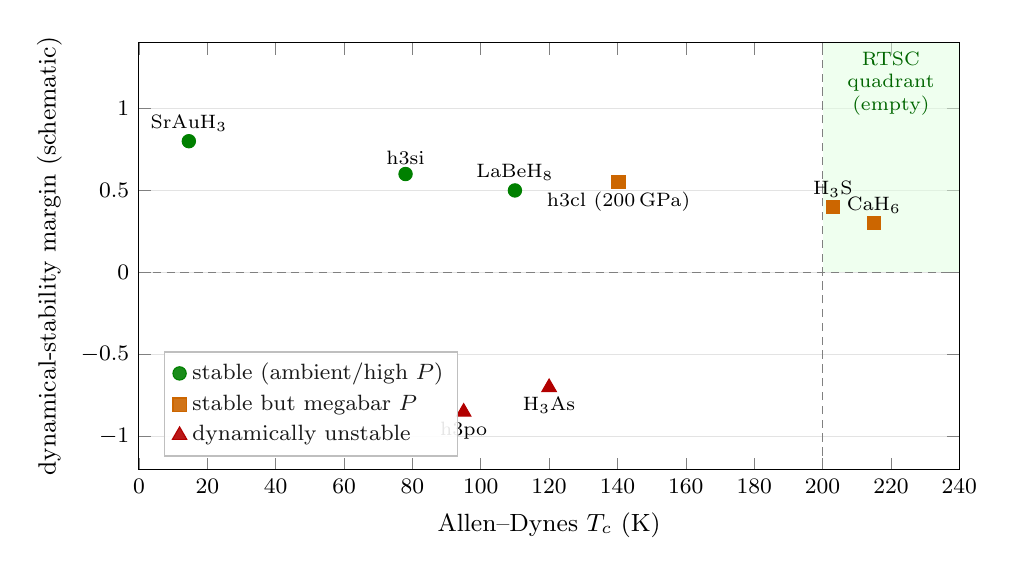
\begin{tikzpicture}
\begin{axis}[
  width=12cm, height=7cm,
  xlabel={Allen--Dynes $T_c$ (K)},
  ylabel={dynamical-stability margin (schematic)},
  xmin=0, xmax=240, ymin=-1.2, ymax=1.4,
  tick label style={font=\footnotesize},
  label style={font=\small},
  ymajorgrids, grid style={gray!22},
  legend pos=south west, legend cell align=left,
  legend style={font=\footnotesize,fill=white,fill opacity=0.9,draw=gray!50},
]
% quadrant guides
\draw[gray,densely dashed] (axis cs:0,0) -- (axis cs:240,0);
\draw[gray,densely dashed] (axis cs:200,-1.2) -- (axis cs:200,1.4);
\fill[green!12,opacity=0.5] (axis cs:200,0) rectangle (axis cs:240,1.4);
\node[font=\scriptsize,green!40!black,align=center] at (axis cs:220,1.15)
  {RTSC\\quadrant\\(empty)};
% stable, low-Tc (ambient)
\addplot[only marks,mark=*,mark size=2.4pt,green!50!black] coordinates {
  (14.6,0.8) (78,0.6) (110,0.5)
};
\addlegendentry{stable (ambient/high $P$)}
% stable, high-Tc, but megabar only
\addplot[only marks,mark=square*,mark size=2.4pt,orange!80!black] coordinates {
  (140.3,0.55) (203,0.4) (215,0.3)
};
\addlegendentry{stable but megabar $P$}
% unstable, high-lambda
\addplot[only marks,mark=triangle*,mark size=3pt,red!70!black] coordinates {
  (120,-0.7) (95,-0.85)
};
\addlegendentry{dynamically unstable}
% labels
\node[font=\scriptsize,anchor=south] at (axis cs:14.6,0.8) {SrAuH$_3$};
\node[font=\scriptsize,anchor=south] at (axis cs:78,0.6) {h3si};
\node[font=\scriptsize,anchor=south] at (axis cs:110,0.5) {LaBeH$_8$};
\node[font=\scriptsize,anchor=north] at (axis cs:140.3,0.55) {h3cl (200\,GPa)};
\node[font=\scriptsize,anchor=south] at (axis cs:203,0.4) {H$_3$S};
\node[font=\scriptsize,anchor=south] at (axis cs:215,0.3) {CaH$_6$};
\node[font=\scriptsize,anchor=north] at (axis cs:120,-0.7) {H$_3$As};
\node[font=\scriptsize,anchor=north] at (axis cs:95,-0.85) {h3po};
\end{axis}
\end{tikzpicture}
\caption{The stability$\leftrightarrow$$T_c$ wall. Each candidate is a
point (Allen--Dynes $T_c$, schematic dynamical-stability margin). Green
discs are ambient/stable but low-$T_c$; orange squares are stable and
high-$T_c$ \emph{but only at megabar pressure}; red triangles are
high-$\lambda$ but dynamically unstable. \textbf{The green-shaded RTSC
quadrant (stable, ambient, $T_c\!>\!200$\,K) is empty} --- the central
honest finding. The schematic stability axis is illustrative
(positive/negative = real/imaginary lowest phonon mode); the $T_c$ axis
values are the recomputed Allen--Dynes numbers of
Table~\ref{tab:hyd-slate}.}
\label{fig:stab-tc}
\end{figure}

% -------------------------------------------------------------------------
\subsection{The §8.9 five-gate matrix --- none clears (b)+(c)+(d)}
\label{app:hyd-fivegate}

Mapping the candidate families onto the five-criterion \texttt{absorbed}
gate of Eq.~\eqref{eq:fivegate} (Appendix~\ref{app:material}) shows the
wall formally: no family clears (b) $T_c\!\ge\!270$\,K, (c) ambient
pressure, and (d) $\ge\!3$-lab replication \emph{simultaneously}.

\begin{table}[h]
\centering
\small
\setlength{\tabcolsep}{6pt}
\begin{tabular}{@{}lccccc l@{}}
\toprule
\textbf{Family} & \textbf{(a) synth} & \textbf{(b) $T_c\!\ge\!270$} &
\textbf{(c) ambient} & \textbf{(d) $\ge\!3$ lab} & \textbf{(e) parity}
& \textbf{absorbed?} \\
\midrule
H$_3$S, LaH$_{10}$ & $\triangle$ DAC & \tierGreen\,$\sim$200 &
  \tierRed\,150\,GPa & \tierGreen\ repl. & $\triangle$ Eliash. & \textbf{never (c)} \\
hexa-rtsc $n{=}6$ & \tierRed\ no recipe & --- & --- & --- & --- & \textbf{never (a)} \\
CSH 2020 claim & \tierGreen\ DAC & \tierGreen\,287\,(claim) &
  \tierRed\,270\,GPa & \tierRed\ retracted & \tierRed & \textbf{never} \\
SrAuH$_3$/ternary & $\triangle$ pred. & \tierRed\,$<$\,160 &
  \tierGreen/$?$ ambient & \tierRed\ 0 lab & $\triangle$ & \textbf{never (b)+(d)} \\
\bottomrule
\end{tabular}
\caption{The hydride families vs the five-gate \texttt{absorbed} criterion
(\S8.9 / Eq.~\ref{eq:fivegate}). Megabar hydrides fail (c) ambient; the
ambient ternaries fail (b) $T_c\!\ge\!270$\,K and (d) replication; the
\emph{spec-only} hexa-rtsc $n{=}6$ family fails (a) --- it is a closed-form
$\sigma\!\cdot\!\tau$ spec with no synthesis route. \textbf{Zero rows clear
(b)+(c)+(d) together}: \texttt{absorbed=true} for an RTSC material is not
reachable until physics supplies a new compound. Every candidate here is
\texttt{absorbed=false}; \textbf{no room-temperature superconductor is
claimed}.}
\label{tab:hyd-fivegate}
\end{table}

% -------------------------------------------------------------------------
\subsection{Breakthrough paths (governance @D d2)}
\label{app:hyd-breakthrough}

The honest conclusion is the one demanded by governance @D d2: an
\emph{empirically-demonstrated wall} is surfaced with concrete breakthrough
paths, never conceded as ``impossible''. The binary-hydride axis is
exhausted for RTSC (Table~\ref{tab:hyd-slate}), but the wall points at
three first-principles paths, recorded here as the forward edge:
\begin{enumerate}\itemsep0.25em
\item \textbf{Ternary cation-decoupling.} In the octahedral X$_2$MH$_6$
  family, the H sublattice that carries $\lambda$ can be \emph{decoupled}
  from the cation sublattice that sets stability. The open question is
  whether a cation choice (Mg$_2$IrH$_6$ $\sim$160\,K predicted ambient,
  Li$_2$CuH$_6$ $\sim$86\,K) keeps the lowest phonon mode real
  ($m\!>\!0$, the (c)-gate) at $1$\,atm while retaining $\lambda$ ---
  the N6 funnel's central DFT test.
\item \textbf{Anharmonic stabilization (SSCHA).} Several binary structures
  flagged \tierRed\ harmonically (h3po, H$_3$As) may be
  \emph{anharmonically} stabilized: the SSCHA self-consistent phonon
  treatment can lift an imaginary harmonic mode to real, as it does for
  metallic hydrogen phases. h3o is already evaluated this way; extending
  SSHA to the \tierRed\ rows is a concrete recompute.
\item \textbf{$\mu^{*}$-robust ranking.} Because the $T_c$ verdict inherits
  $\mu^{*}$ uncertainty (Appendix~\ref{app:elph}), a candidate that clears
  $T_c\!>\!200$\,K \emph{robustly} across $\mu^{*}\!\in\![0.10,0.13]$ is a
  stronger funnel pass than one that clears only at $\mu^{*}=0.10$ ---
  a re-ranking of the existing slate at no new DFT cost.
\end{enumerate}
None of these flips \texttt{absorbed=true} (that stays wet-lab, @D d5); they
are candidate-filtering and wet-lab-prioritization moves. They are recorded
as open milestones, not closed --- the wall is a forward edge, not a
terminus. \textbf{No room-temperature superconductor is claimed here.}
